\documentclass{beamer}

\usepackage[ngerman]{babel}
\usepackage[utf8]{inputenc}
\usepackage{hyperref}
\usepackage{eurosym}

\mode<presentation>{
	\definecolor{LogoRed}{RGB}{219,00,31}
	\definecolor{LogoGray}{RGB}{86,86,80}
	
	\useoutertheme[width=2.1cm]{sidebar}
	\useinnertheme{rounded}
	\setbeamercolor{normal text}{fg=black,bg=white}
	\setbeamercolor{palette sidebar primary}{use=normal text,fg=normal text.fg}
	\setbeamercolor{title}{fg=LogoRed}
	\setbeamercolor{frametitle}{fg=LogoRed}
	\setbeamercolor{structure}{fg=LogoRed}
	\setbeamercolor{section in sidebar}{fg=LogoRed}
	\setbeamercolor{subsection in sidebar}{fg=LogoRed}
	
	\usefoottemplate{\vbox{\tinycolouredline{LogoGray!25}{\hspace{4pt}\hspace{15pt}\insertdate\hfill\insertshortinstitute\hfill \insertframenumber{}/\inserttotalframenumber}}}
	
	\setbeamertemplate{section in toc}{\inserttocsectionnumber.~\inserttocsection\par}
	\setbeamertemplate{subsection in toc}{\hspace*{2em}\inserttocsectionnumber.\inserttocsubsectionnumber~\inserttocsubsection}
	\AtBeginSubsection[] {
		\begin{frame}<beamer>
			\frametitle{Outline}
			\tableofcontents[currentsection,sectionstyle=show/show,subsectionstyle=show/shaded/hide]
		\end{frame}
	}
}

\title{Erstsemestereinführung WS 2015/16}
\author[Diana Irmscher]{Diana Irmscher\\\texttt{irmscher@fs.cs.hm.edu}}
\institute[Fachschaft 07]{Fachschaft 07\\Fakultät für Informatik und Mathematik\\Hochschule für angewandte Wissenschaften München}
\logo{
\includegraphics[height=1.0cm]{logo_hm.png}}
\date{\today}

\setbeamertemplate{navigation symbols}{}

\begin{document}
	\maketitle
	
	\section{Begrüßung}
	
	\begin{frame} %% Die Vortragenden stellen sich vor
		\frametitle{Vorstellung Fachschaftsleitung}
		
		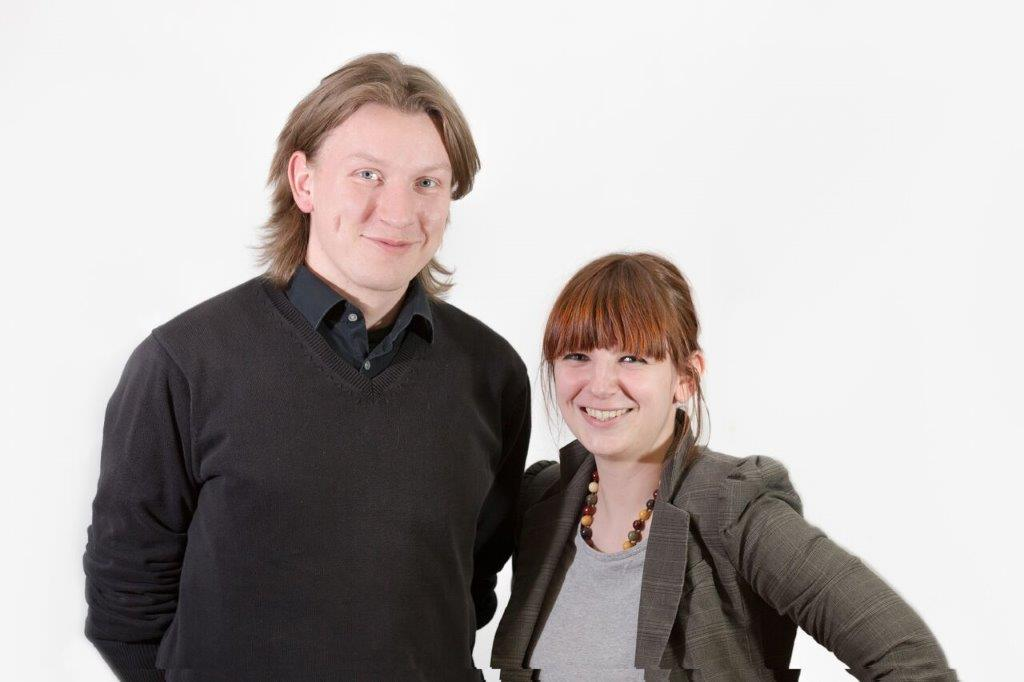
\includegraphics[width=0.9\textwidth]{diana_matti.jpg}
		\begin{columns}
			\column{.47\textwidth}

			\textbf{Mathias Duve}
			\\
			Wirtschaftsinformatik, Bachelor
			\column{.47\textwidth}
			\textbf{Diana Irmscher}
			\\
			Informatik, Bachelor
		\end{columns}

	\end{frame}
	
	\begin{frame} %% Agenda zeigen, was noch ansteht
		\frametitle{Agenda}
		\tableofcontents
	\end{frame}
	
	\section{Dekanat der Fakultät 07}
	
	\begin{frame} %% Der Dekan wird vorgestellt
		\frametitle{Das Dekanat der Fakultät 07}
			\begin{columns}
                \column{.67\textwidth}
                \begin{itemize}
                	\item Dekan: Prof. Dr. Jochen Hertle
                	\bigskip
                	\bigskip
                	\bigskip
                	\item Prodekan: Prof. Dr. Veronika Thurner
                	\bigskip
                	\item Studiendekan: Prof. Dr. Axel Böttcher
                \end{itemize}
                \column{.67\textwidth}
                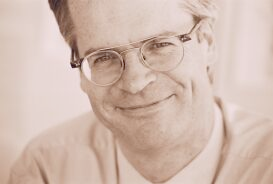
\includegraphics[width=0.3\textwidth]{jochen-hertle.png} \\
                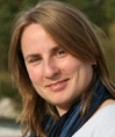
\includegraphics[width=0.3\textwidth]{Prof_Thurner.jpg} \\
                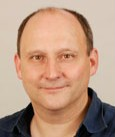
\includegraphics[width=0.3\textwidth]{boettcher.jpg}
			\end{columns}
		%% was ist mit dem Rest, fasse ich das gleich hier ein?
    \end{frame}
    
    \begin{frame} %% Der Dekan wird vorgestellt
    	\frametitle{Grußwort des Dekans}
    	\center
    	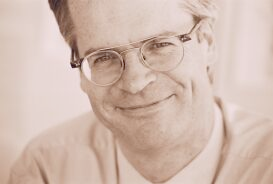
\includegraphics[width=0.7\textwidth]{jochen-hertle.png}
    	\\
    	\textbf{Prof. Dr. Jochen Hertle}
    \end{frame}
    
    \begin{frame} %% Der Prodekan wird vorgestellt
    	\frametitle{Prodekanin}
    	\begin{columns}
    		\column{.17\textwidth}
    		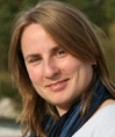
\includegraphics[width=1.0\textwidth]{Prof_Thurner.jpg}
    		\column{.67\textwidth}
    		\textbf{Prof. Dr. Veronika Thurner}
    		\begin{itemize}
    			\item Prodekanin der Fakultät 07
    			\item Frauenbeauftragte der Fakultät 07
    			\item Ansprechpartnerin für
    			\begin{itemize}
    				\item Studierende mit Kind
    				\item Gender
    				\item Bayern Mentoring für Studierende
    			\end{itemize}
    			\bigskip
    			\item Kontakt
    			\begin{itemize}
    				\item R2.039
    				\item thurner@hm.edu
    				\item Sprechstunde
    				\begin{itemize}
    					\item donnerstags, 09:00 Uhr
    					\item Außerhalb der Vorlesungszeit nach Vereinbarung per E-Mail
    				\end{itemize}
    			\end{itemize}
    		\end{itemize}
    	\end{columns}
    \end{frame}
    
    \begin{frame} %% Der Studiendekan wird vorgestellt
    	\frametitle{Studiendekan}
    	\begin{columns}
    		\column{.17\textwidth}
    		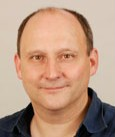
\includegraphics[width=1.0\textwidth]{boettcher.jpg}
    		\column{.67\textwidth}
    		\textbf{Prof. Dr. Axel Böttcher}
    		\begin{itemize}
    			\item Studiendekan der Fakultät 07
    			\bigskip
    			\item Kontakt
    			\begin{itemize}
    				\item R4.027
    				\item thurner@hm.edu
    				\item Sprechstunde
    				\begin{itemize}
    					\item montags, 14:00 Uhr
    				\end{itemize}
    			\end{itemize}
    		\end{itemize}
    	\end{columns}
    \end{frame}
    
    \section{Auftaktveranstaltung}
    
    \begin{frame} 
    	\frametitle{Auftaktveranstaltung}
    	\textbf{Freitag, 02.10.2015}\\
    	Ziel:
    	\begin{itemize}
    		\item Ermittlung Ihrer Kompetenzen zum Studienbeginn
    	\end{itemize}
    	\bigskip
    	Nutzen für Sie als Studierende
    	\begin{itemize}
    		\item eigenes Kompetenzprofil bewusst machen
    		\item Verbesserungspotenzial frühzeitig erkennen
        \end{itemize}
        \bigskip
        Nutzen für die Lehrende der Fakultät
        \begin{itemize}
        	\item Feststellen, wo noch Fragen sind
        	\item Einstellung auf die Studiengruppe schon zu Beginn des Semesters
        \end{itemize}
        Wir wollen Sie weder langweilen noch überfordern!
    \end{frame}
    
    \begin{frame} 
    	\frametitle{Auftaktveranstaltung}
    	\begin{columns}
    		\column{.47\textwidth}
    		Studiengruppe \textbf{IB1A}
    		\begin{itemize}
    			\item 11:45 Uhr
    			\item Raum 1.006
    		\end{itemize}
    		\bigskip
    		Studiengruppe \textbf{IB1C}
    		\begin{itemize}
    			\item 08:15 Uhr
    			\item Raum R0.007
    			\item Thurner / Schiffner
    		\end{itemize}
    		\bigskip
    		Studiengruppen \textbf{IC1}, \textbf{GO1}
    		\begin{itemize}
    			\item 8:15 Uhr
    			\item Raum R0.011
    			\item Böttcher
    		\end{itemize}
    		\column{.47\textwidth}
    		Studiengruppe \textbf{IF1A}
    		\begin{itemize}
    			\item 12:30 Uhr
    			\item Raum R1.007
    			\item Hobelsberger
    		\end{itemize}
    		\bigskip
    		Studiengruppe \textbf{IF1B}
    		\begin{itemize}
    			\item 12:30 Uhr
    			\item Raum R2.007
    			\item Orehek
    		\end{itemize}
    	\end{columns}
    \end{frame}
    
    \section{Hochschulgemeinde}
    
    \begin{frame} 
    	\frametitle{Hochschulgemeinde}
    	
\includegraphics[width=0.9\textwidth]{ekhg.jpg}
    	\\
		\url{www.ekhg.hm.edu}
		\\
		\url{www.facebook.com/ekhgmuenchen}
    \end{frame}
    
    \begin{frame} 
    	\frametitle{Hochschulgemeinde}
    	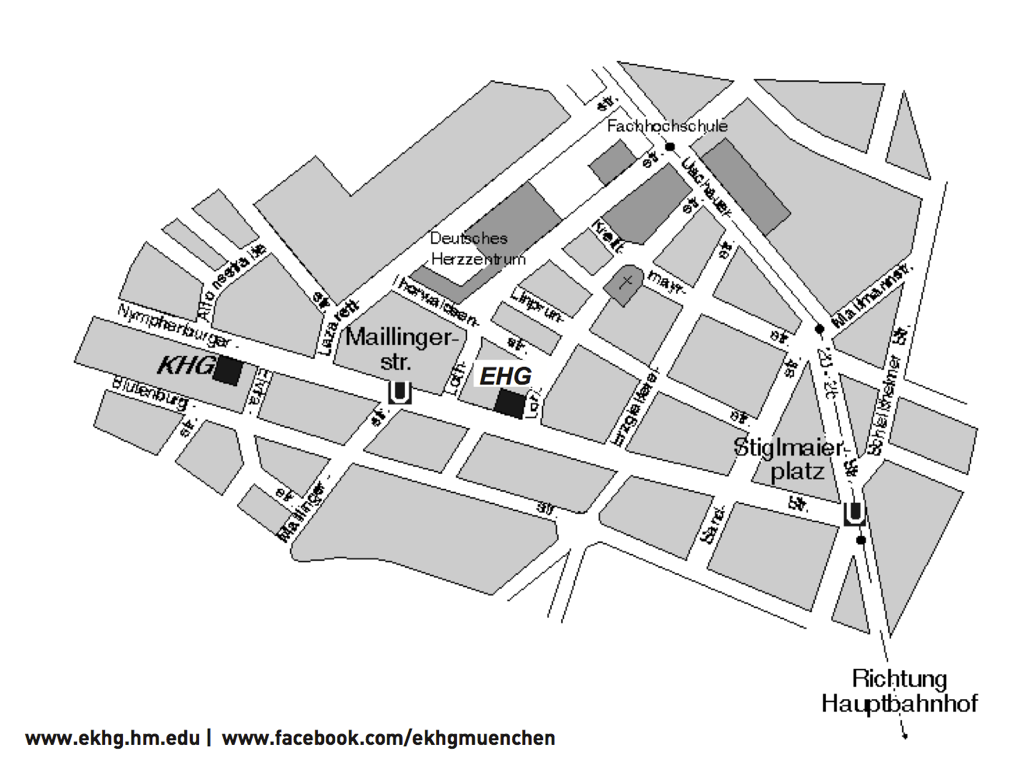
\includegraphics[width=1\textwidth]{anfahrt-ekhg.png}
    \end{frame}
    
    \section{Ansprechpartner}
    
    \begin{frame} 
    	\frametitle{Sekretariat der Fakultät 07}
    	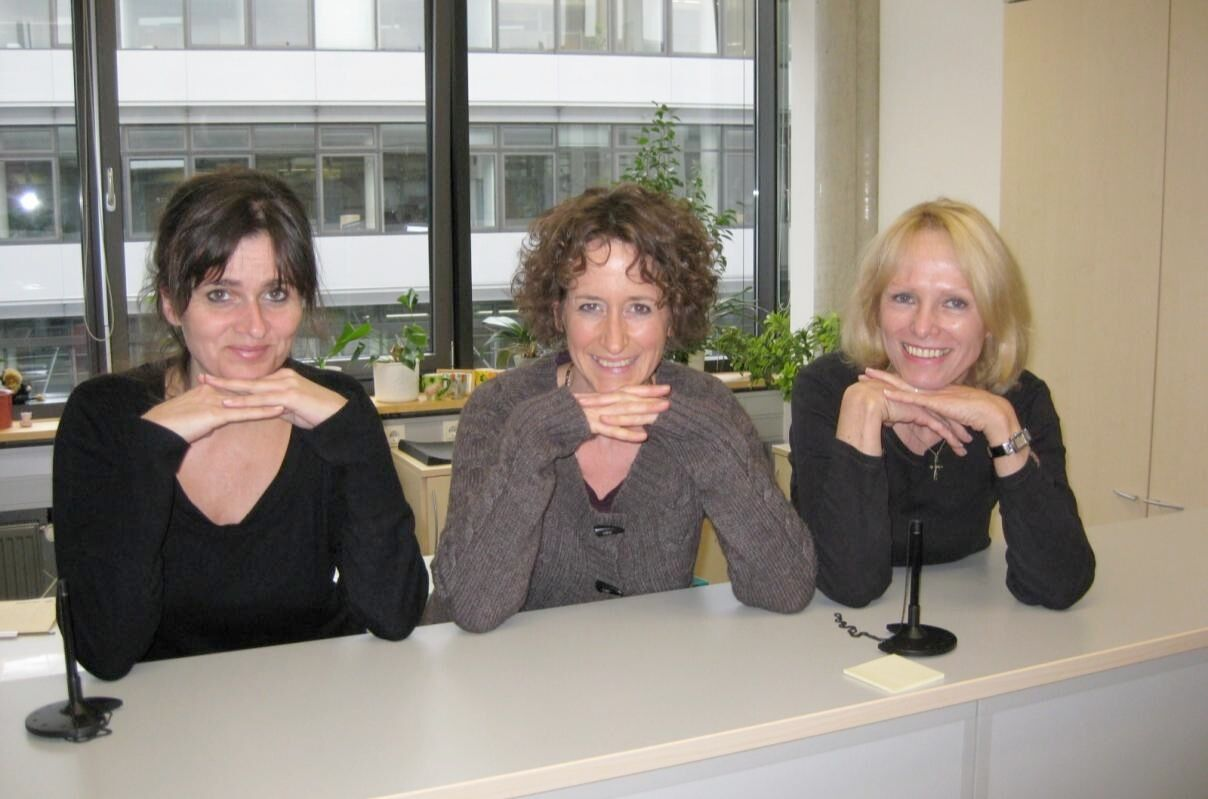
\includegraphics[width=0.94\textwidth]{sekretariat.jpg}
    	\begin{columns}[t]
    		\column{.27\textwidth}
    		\textbf{Christine Bunge}
    		\column{.27\textwidth}
    		\textbf{Michaela Rambausek}
    		\column{.27\textwidth}
    		\textbf{Helene Dietz}
    	\end{columns}
    \end{frame}
    
    \begin{frame} 
        \frametitle{Fachschaft der Fakultät 07}
        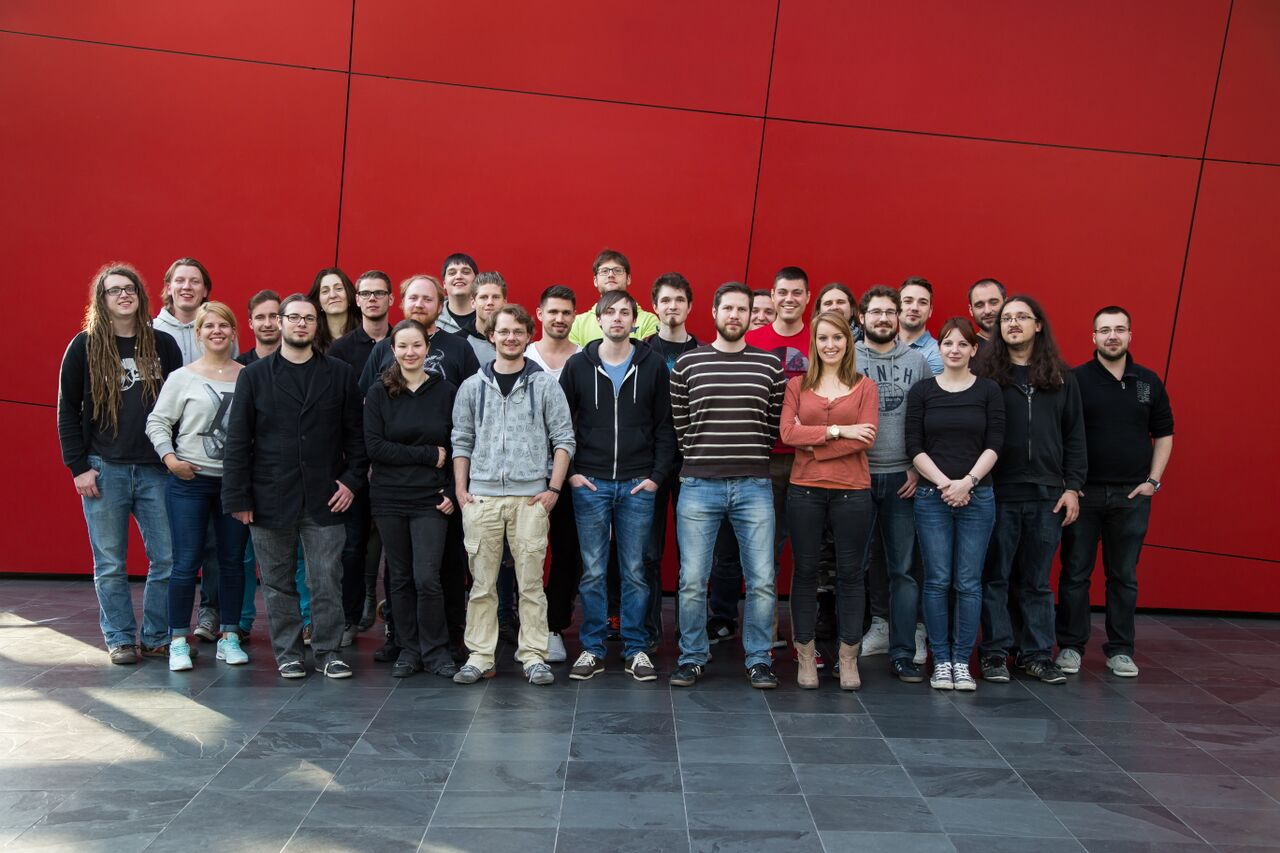
\includegraphics[width=0.94\textwidth]{fachschaft.jpg}
        \\
        \textbf{Fachschaft im letzten Semester}
    \end{frame}
    
    \begin{frame}[t]
    	\frametitle{Was macht die Fachschaft?}
    	
    	\begin{itemize}
    		\item Ansprechpartner für Fragen zum Studium
    		\item Hochschulpolitik:
    		\begin{itemize}
    			\item Fakultätsrat
    			\item Paritätische Kommission
    		    \item Studentisches Parlament
    		\end{itemize}
    		\item Social Media
    		\begin{itemize}
    			\item Facebook-Seite: www.facebook.com/fachschaft07
    			\item Facebook-Gruppe: Studenten Fakultät 07 HM
    		\end{itemize}
    		\item Skriptendruck
    		\item Vorkurs
    		\item Erstsemesterveranstaltung
    		\item Studentische Vollversammlung
    		\item RetroGaming Abend
    		\item Speeddating (Firmenkontakte)
    		\item Absolventenfeier
    	\end{itemize}
    \end{frame}
    
    \begin{frame}[t]
    	\frametitle{ErstiGuide}
    	Wir haben wichtige Informationen für Erstsemester in einem Guide für euch zusammengestellt.\\
    	\bigskip
    	Download unter \url{fs.cs.hm.edu}\\
    	\center
    	
\includegraphics[width=0.3\textwidth]{erstiguide.jpg}
    \end{frame}
    
    \begin{frame}[t]
    	\frametitle{Hochschulpolitik}
    	Die gewählten Vertreter für euch:\\
    	\bigskip
    	\textbf{Fakultätsrat}
    	\bigskip
    	\begin{columns}[t]
    		\column{.21\textwidth}
    		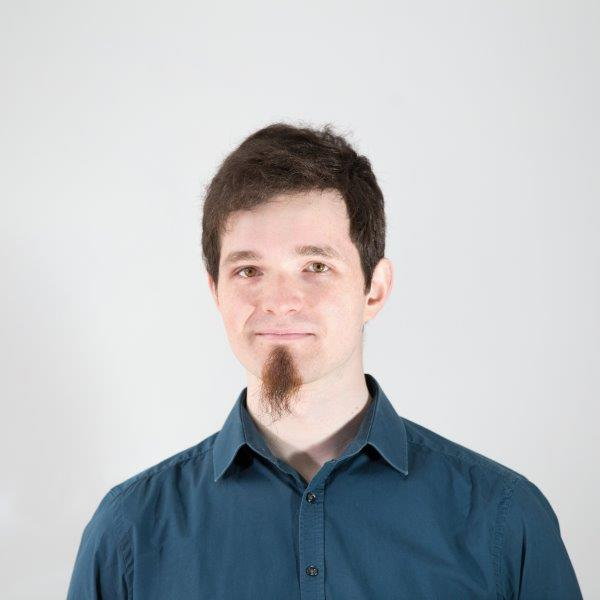
\includegraphics[width=0.9\textwidth]{fabian.jpg}
    		\\
    		\textbf{Fabian Trampusch}
    		\column{.21\textwidth}
    		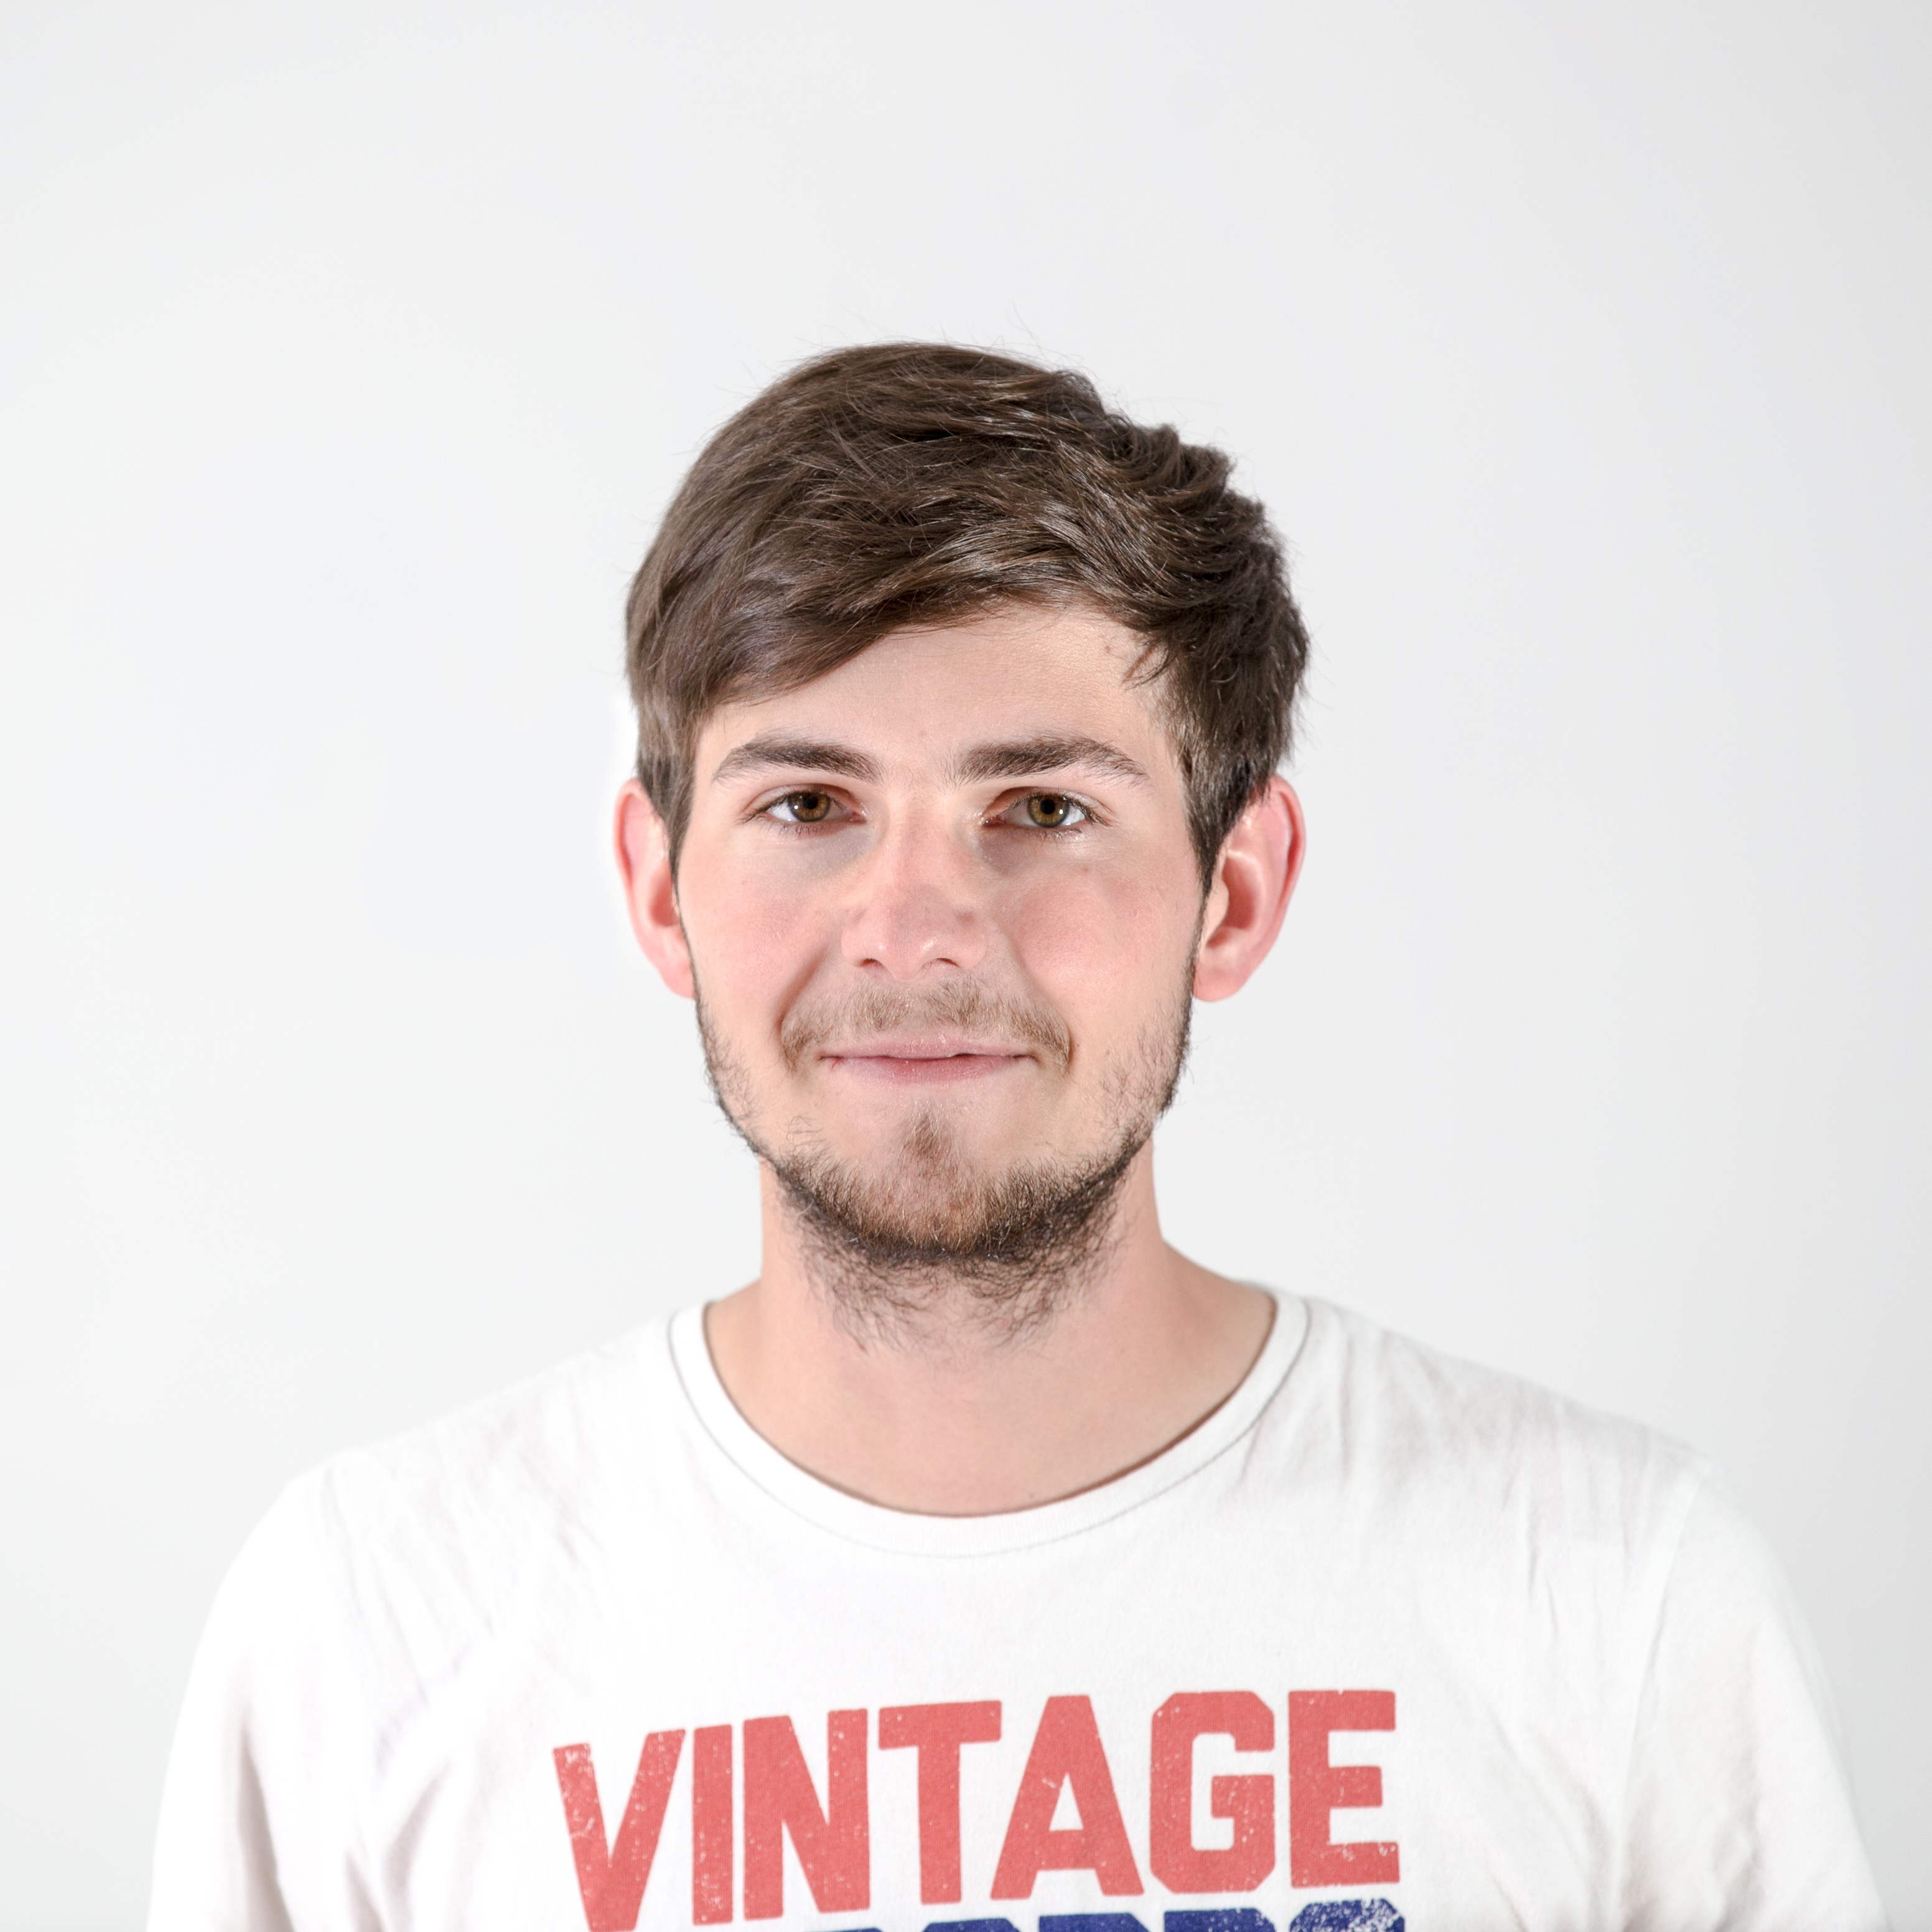
\includegraphics[width=0.9\textwidth]{anselm.jpg}
    		\\
    		\textbf{Anselm Binniger}
    	\end{columns}
    	\begin{columns}[t]
    		\column{.21\textwidth}
    		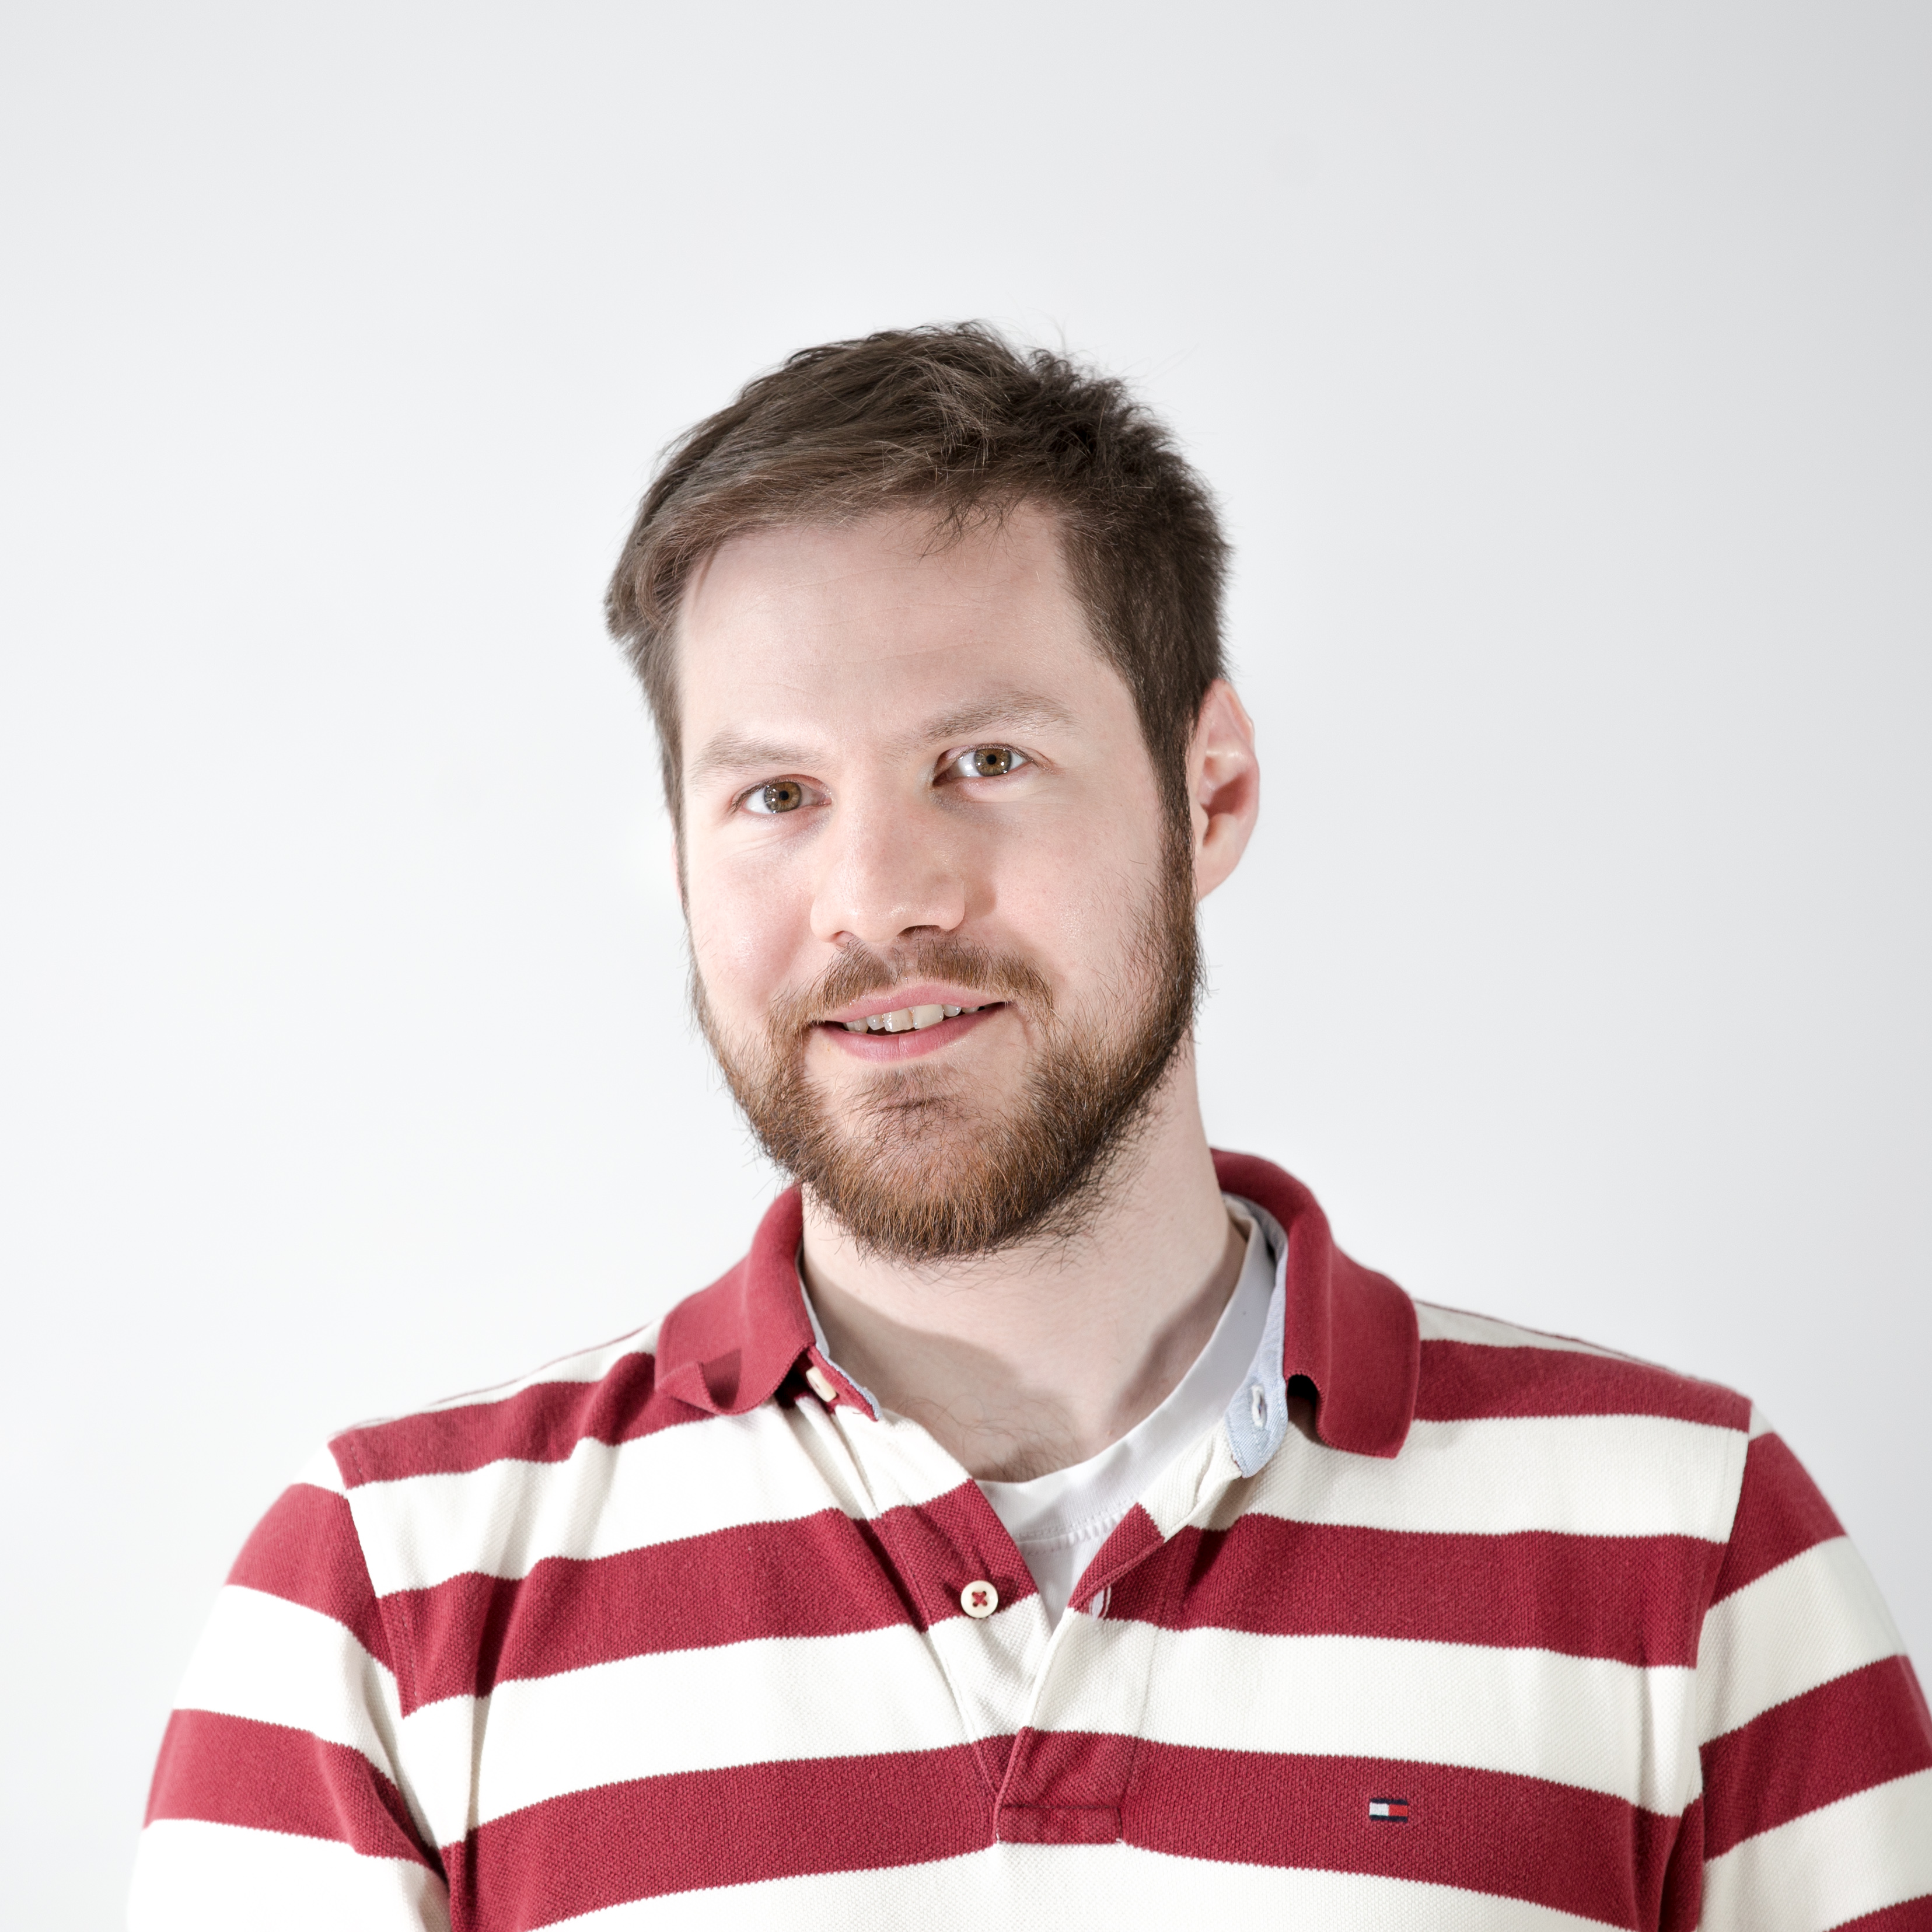
\includegraphics[width=0.9\textwidth]{ersin.jpg}
    		\\
    		\textbf{Ersin Ötztürk}
    		\column{.21\textwidth}
    		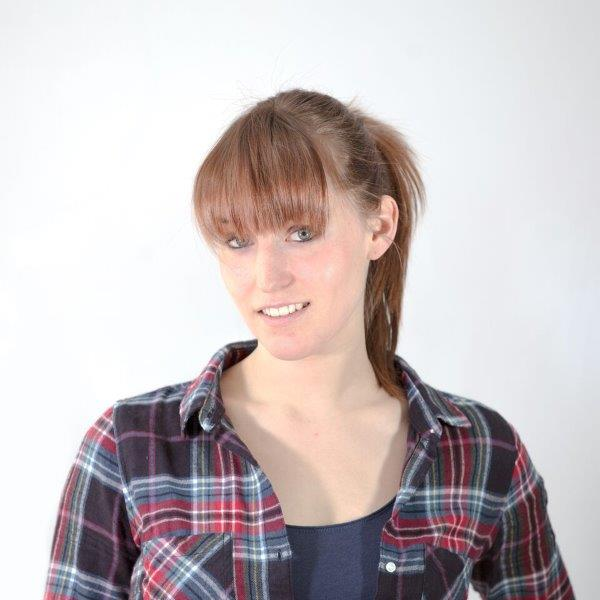
\includegraphics[width=0.9\textwidth]{nicole.jpg}
    		\\
    		\textbf{Nicole Behrens}
    	\end{columns}
    \end{frame}
    
    \begin{frame}[t]
    	\frametitle{Hochschulpolitik}
    	\textbf{Studentisches Parlament}
    	\bigskip
    	\begin{columns}[t]
    		\column{.40\textwidth}
    		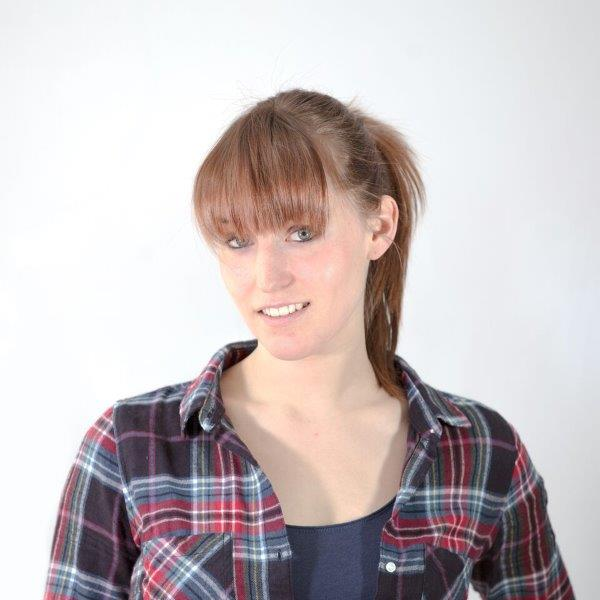
\includegraphics[width=0.9\textwidth]{nicole.jpg}
    		\\
    		\textbf{Nicole Behrens}
    	\end{columns}
    \end{frame}
    
    \begin{frame}[t]
    	\frametitle{Hochschulpolitik}
    	\textbf{Paritätische Kommision}
    	\bigskip
    	\begin{columns}[t]
    		\column{.40\textwidth}
    		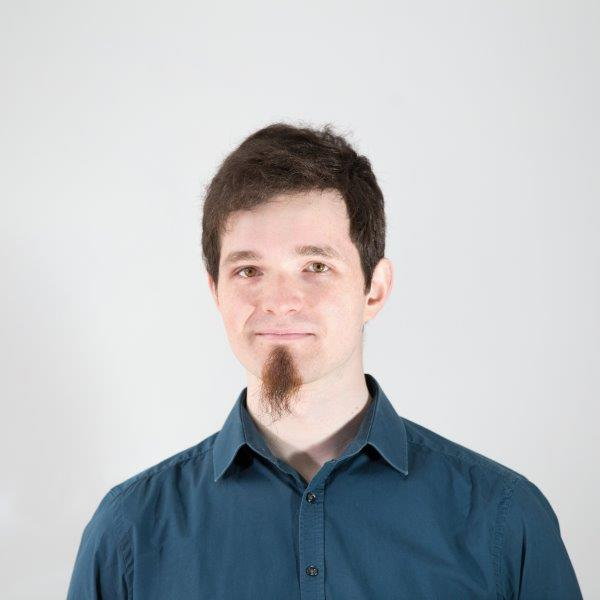
\includegraphics[width=0.9\textwidth]{fabian.jpg}
    		\\
    		\textbf{Fabian Trampusch}
    		\column{.40\textwidth}
    		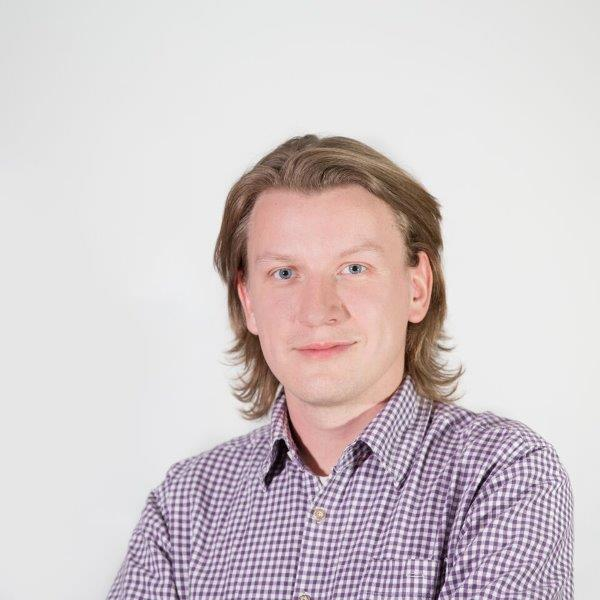
\includegraphics[width=0.9\textwidth]{matti.jpg}
    		\\
    		\textbf{Mathias Duve}
    	\end{columns}
    \end{frame}
    
    \begin{frame}[t]
    	\frametitle{Studentische Vertretung}
    	\center
    	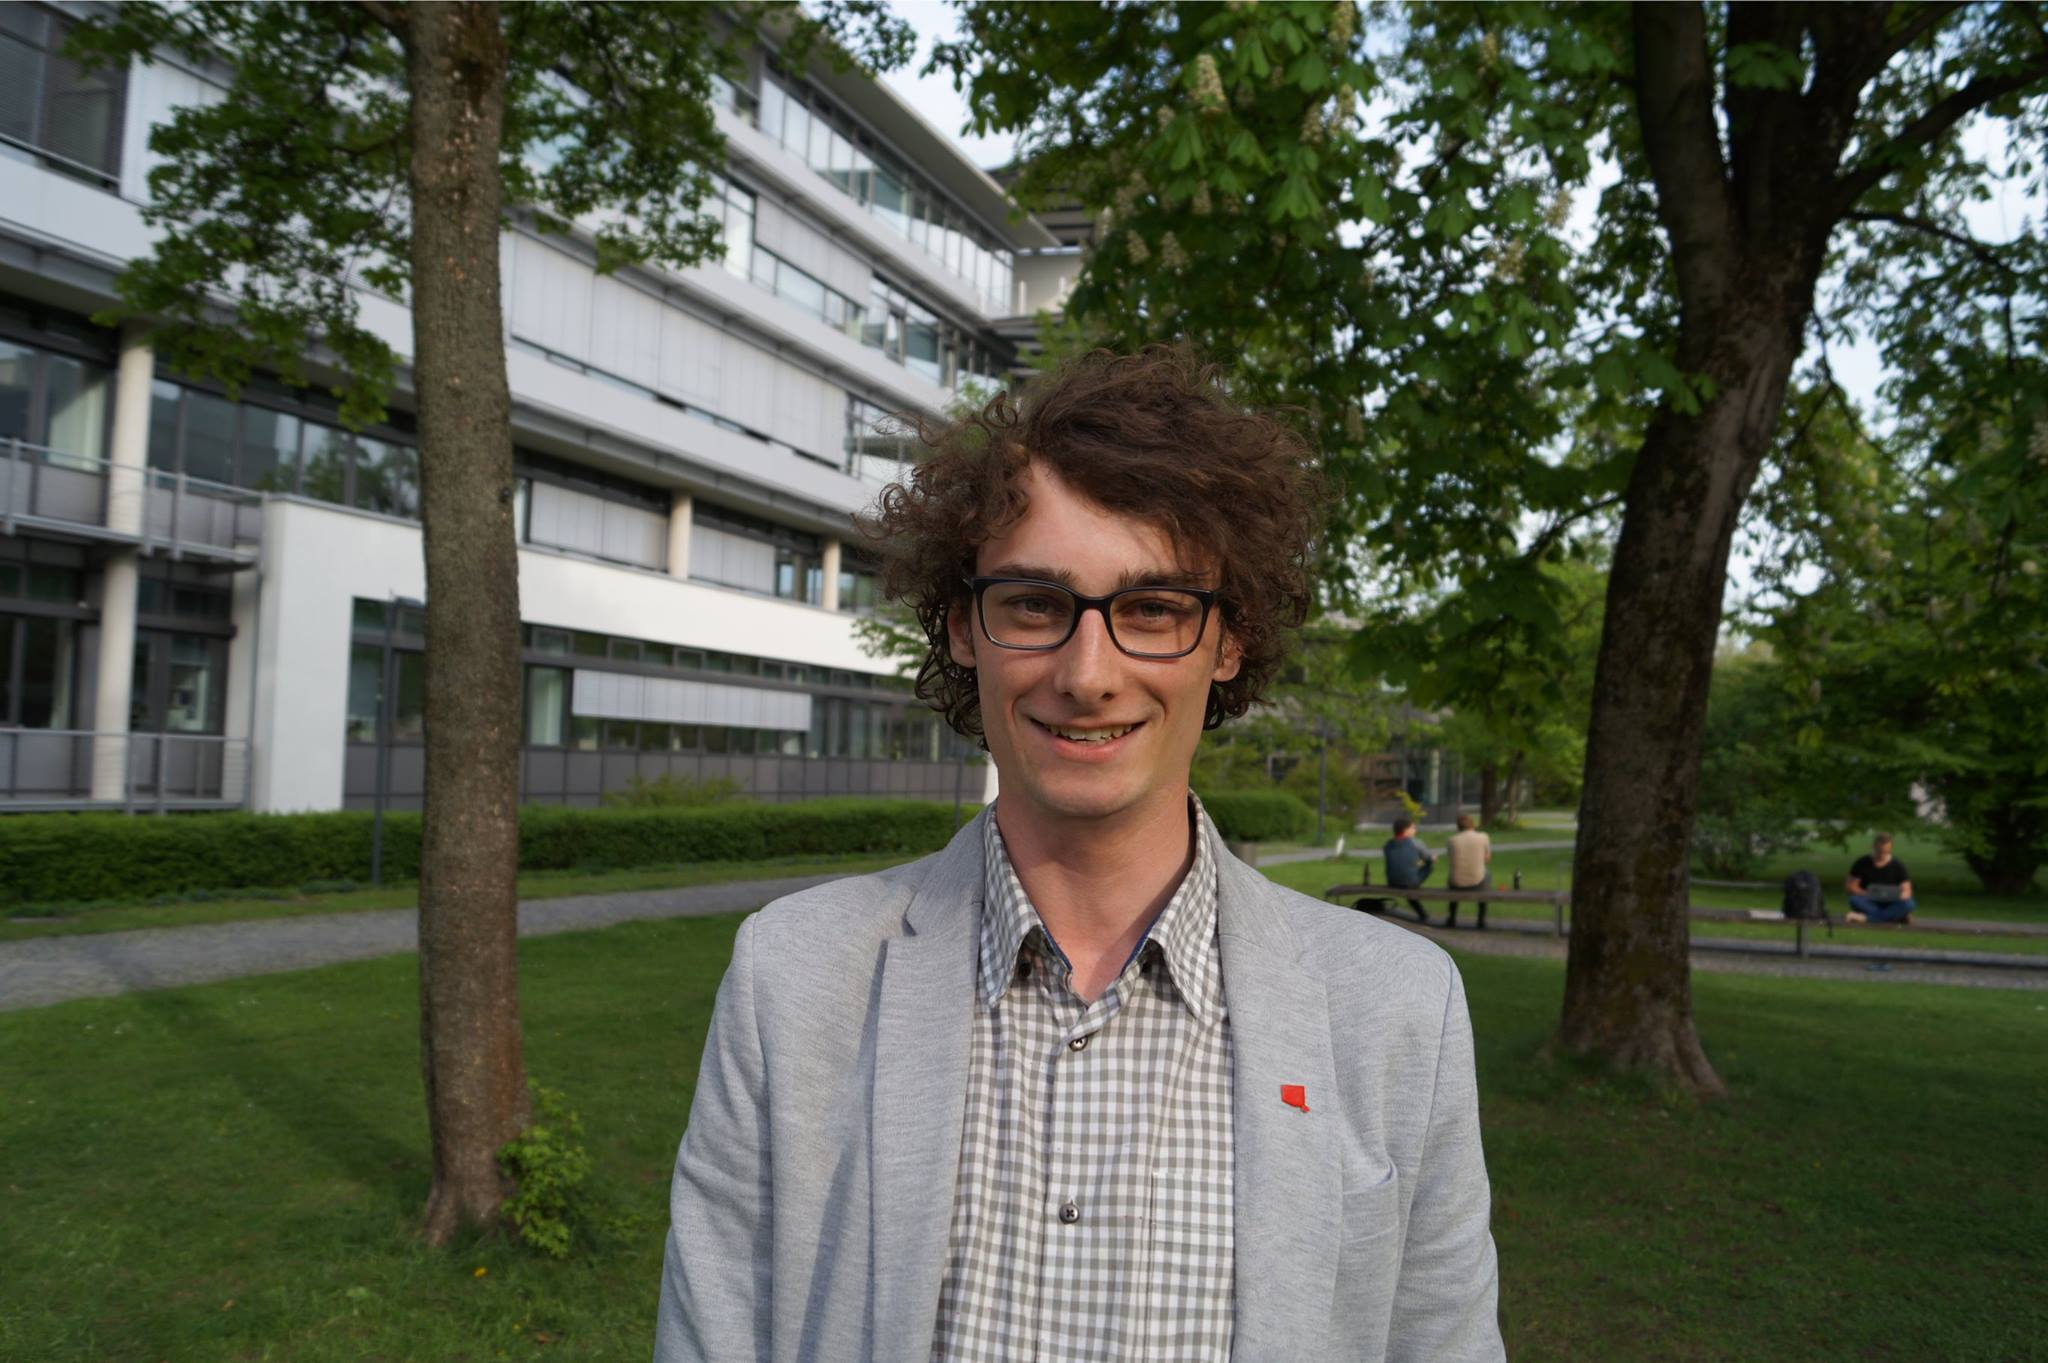
\includegraphics[width=0.8\textwidth]{pittruff.jpg}
    	\\
    	\textbf{Constantin Pittruff}
    \end{frame}
    
    \section{Studium}
    
    \begin{frame}[t]
    	\frametitle{Accounts}
    	\qquad
    	
\includegraphics[width=0.08\textwidth]{xmail.jpg}
    	\qquad
    	
\includegraphics[width=0.1\textwidth]{primuss.jpg}
    	\qquad
    	
\includegraphics[width=0.1\textwidth]{moodle.png}
    	\qquad
    	
\includegraphics[width=0.1\textwidth]{eduroam.png}
    	\qquad
    	
\includegraphics[width=0.2\textwidth]{lrz.png}
    	\begin{itemize} 
    		\item Hochschul-Account
    		\begin{itemize}
    			\item Mail-Postfach unter \\ \url{https://xmail.mwn.de}
    			\item PRIMUSS System unter \url{www.hm.edu/online-services}
    		\end{itemize}
    		\pause
    		\item Moodle (E-Learning-Plattform)
    		\begin{itemize}
    			\item Mail-Postfach unter \url{moodle.hm.edu}
    		\end{itemize}
    		\pause
    		\item Eduroam (WLAN)
    		\begin{itemize}
    			\item \url{www.lrz.de/services/netz/mobil/wireless/}
    		\end{itemize}
    		\pause
    		\item LRZ (VPN/WLAN)
    		\begin{itemize}
    			\item \url{www.lrz.de/services/netz/mobil/vpn/}
    		\end{itemize}
    	\end{itemize}
    \end{frame}
    
    \begin{frame}[t]
    	\frametitle{Accounts}
    	\begin{itemize}
    		\item FK07-Kennung
    		\begin{itemize}
    			\item ifw-Account, z.B. ifw12345
    			\item Laborrechner
    		\end{itemize}
    	\end{itemize}
    	\pause
    	\flushright
    	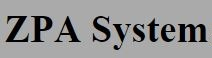
\includegraphics[width=0.3\textwidth]{zpa.jpg}
    	\begin{itemize}
    		\item ZPA-System
    		\begin{itemize}
    			\item \url{w3-o.cs.hm.edu/zpa/}
    			\item Zeitplan einsehen, um keine Termine zu verpassen
    			\item \footnotesize{\url{http://w3-o.cs.hm.edu/mediapool/zpa/zpa_info.html}}
    			\item \normalsize{Anmeldung mit FK07-Account}$  $
    			\item Anmeldung für FWP-Fächer (mit und ohne Praktika),
    			praxisbegleitenden Unterricht,
    			Blockunterricht,
    			Praktika zu bestimmten Vorlesungen und
    			Seminaren
    		\end{itemize}
    	\end{itemize}
    \end{frame}
    
    \begin{frame}
    	\frametitle{Vorstellung des ZPA}
    	\begin{columns}[t]
    		\column{.17\textwidth}
    		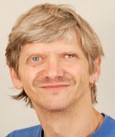
\includegraphics[width=1.0\textwidth]{vogler.jpg}
    		\\
    		\textbf{Thomas Vogler}
    		\column{.67\textwidth}
    		\begin{itemize}
    			\item ZPA System (Wartung und Programmierung)
    			\item DreamSpark Administrator
    	    \end{itemize}
    	\end{columns}
    \end{frame}
    
    \begin{frame}
    	\frametitle{Allgemeinwissenschaftliche Wahlpflichtfächer}
    	\begin{itemize}
    		\item Fakultät 13
    		\item Liste der Module unter: 
    		\begin{itemize}
    			\item \url{https://w3-mediapool.hm.edu/mediapool/media/fk13/fk13_lokal/pdfaw/aaa_VV_WS1516.pdf}
    		\end{itemize}
    		\item nach eigenem Interesse auswählen
    	\end{itemize}
    \end{frame}
    
    \begin{frame}[t]
    	\frametitle{Termine: Wahl der AW-Fächer}
    	\flushright
    	
\includegraphics[width=0.3\textwidth]{primuss.jpg}
    	\begin{itemize}
    		\item \textbf{Wahl der AW-Fächer}
    		    \begin{itemize}
    		    	\item 17.09. - 02.10.2015: Belegung 1. Los-Durchgang
    		    	\item 05.10.2015: Bekanntgabe des 1. Los-Durchgangs
    		    	\item 05.10. - 06.10.2015: Belegung 2. Los-Durchgang
    		    	\item 07.10.2015: Bekanntgabe des 2. Los-Durchgangs
    		    	\bigskip
    		    	\item Anmeldung im PRIMUSS System der Hochschule
    		    	\item \url{www.hm.edu/online-services}
    		    \end{itemize}
    	\end{itemize}
    \end{frame}

    \begin{frame}
    	\flushright
    	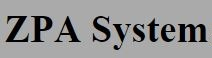
\includegraphics[width=0.3\textwidth]{zpa.jpg}
    	\frametitle{Termine: Wahl der Vorlesungen und Praktika}
    	\begin{itemize}
    		\item \textbf{Vorlesungen / Praktika}
    		\begin{itemize}
    			\item zum Ende des Semesters (für das folgende Semester)
    			\item ZPA-System
    			\item \url{https://w3-o.cs.hm.edu/zpa}
    			\item ACHTUNG: zum Teil in der Prüfungszeit!
    		\end{itemize}
    	\end{itemize}
    \end{frame}

    \begin{frame}
    	\frametitle{Termine: Anmeldung zur Prüfung}
    	\flushright
    	
\includegraphics[width=0.3\textwidth]{primuss.jpg}
    	\begin{itemize}
    		\item \textbf{Prüfungen}
    		\begin{itemize}
    			\item 02.11.2015 – 16.11.2015
    			\item im PRIMUSS System der Hochschule
    			\item \url{www.hm.edu/online-services}
    		\end{itemize}
    		\item Anmeldung zur Prüfung ist nicht verbindlich
    	\end{itemize}
    \end{frame}
    
    \begin{frame}
    	\frametitle{Termine: Rückmeldung zum nächsten Semester}
    	\begin{itemize}
    		\item 15.01.2016 – 14.02.2016
    		\begin{itemize}
    			\item im PRIMUSS System der Hochschule
    			\item \url{www.hm.edu/online-services}
    		\end{itemize}
    		\pause
    		\item Bestätigung, dass Studium fortgesetzt wird
    		\pause
    		\item setzt sich zusammen aus:
    	\end{itemize}
    	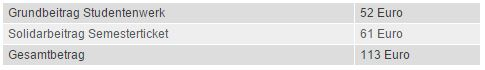
\includegraphics[width=1\textwidth]{rueckmeldung.jpg}
    	\pause
    	\begin{itemize}
    		\item IsarCard Semester kann für \EUR{152} ergänzt werden
    		\item Informationen dazu: \footnotesize{\url{http://www.mvv-muenchen.de/de/tickets-preise/tickets/schule-ausbildung-und-studium/mvv-semesterticket/}}
    	\end{itemize}
    \end{frame}
    
     \begin{frame}[t]
     	\frametitle{Tipps für's Studium}
     	\begin{itemize}
     		\item Lerngruppen
     		\pause
     		\item Wahl des Praktikumspartners
     		\pause
     		\item Organisation des Studiums: Prüfungen schieben ist immer schlecht
     		\pause
     		\item eigenes Notebook ist empfehlenswert
     		\pause
     		\item Bücher bekommt man alle in der Bibliothek \url{bib.hm.edu}
     	\end{itemize}
     \end{frame}
     
     \begin{frame}[t]
     	\frametitle{Tipps für's Studium}
     	\begin{itemize}
     		\item Unterlagen, Skripte 
     		\begin{itemize}
     			\item Moodle
     			\item Skriptensammlung der Fachschaft
     			\item Skriptenbestellung der Fachschaft
     		\end{itemize}
     		\pause
     		\item Website der Fachschaft\\ \url{fs.cs.hm.edu}
     		\pause
     		\item Android-App der Fachschaft\\ \url{play.google.com/store/apps/details?id=com.fk07}
     		\pause
     		\item iOS-App der Fachschaft\\
     		in Arbeit	
     	\end{itemize}
     \end{frame}
     
     \begin{frame}[t]
     	\frametitle{In welcher Studiengruppe bin ich?}
     	\begin{itemize}
     		\item
     	\end{itemize}
     \end{frame}
     
     \begin{frame}
     	\frametitle{Schwarzes Brett}
     	\begin{itemize}
     		\item alle wichtigen Informationen im Semester
     		\item kurzfristige News, z.B. wenn Vorlesung ausfällt, Termine verschoben werden, etc.
     		\item Link: \footnotesize{\url{http://www.cs.hm.edu/aktuelles/infoscreen/index.de.html}}
     		\item \normalsize{gefiltert von der Fachschaft:} \footnotesize{\url{http://fs.cs.hm.edu/infos/schwarzes-brett/}}
     	\end{itemize}
     \end{frame}
     
     \section{Events}
     
     \begin{frame}[t]
     	\frametitle{Semester Opening Party}
     	\textbf{RED DICE - 01.10.2015 - Cafe Cord Lounge - 21 Uhr}
     	
\includegraphics[width=1\textwidth]{RedDice.jpg}
     	\begin{itemize}
     		\item Abendkasse \EUR{5}
     		\item vergünstigter Eintritt \EUR{3}
     		\item Vorverkauf in der Fachschaft
     		\item Link: \footnotesize{\url{https://www.facebook.com/events/319849874805466}}
     	\end{itemize}
     \end{frame}
     
     \section{Abschluss}
     
     \begin{frame}
     	\center \textbf{Habt ihr noch Fragen?}
     \end{frame}
    
    \begin{frame}
    	\center \textbf{Danke für eure Aufmerksamkeit!}
    	\\
    	\bigskip
    	Die Fachschaft wünscht euch einen guten Start ins Studium!\\
    	\bigskip
    	Und nicht vergessen: wir stehen euch immer mit Rat und Tat zur Seite!\\ 
    	\textless3
    \end{frame}
    
\end{document}